\documentclass[12pt]{beamer}
\usepackage[utf8x]{inputenc}
\usepackage{amsmath}
\usepackage{graphics}
\usepackage{bm}
\title{Stofftransport \& Reaktionsgleichungen}
\subtitle{Projekt zur Vorlesung Numerische Simulation WS16/17}
\author{P.~Buchfink \and E.~Ott \and M.~Schleicher}
\usetheme{Berkeley}
\usecolortheme{crane}
\subject{Simulation Technology}

\begin{document}

  \begin{frame}
    \titlepage
  \end{frame}

  \section{RAD-Gleichungen}
    \begin{frame}
    \frametitle{Wiederholung: Diffusions-Advektionsgleichung}
    \begin{center}
    \begin{tabular}{ c c }
	Diffusion & Advektion \\
	$\frac{\partial s(t,\vec{x})}{\partial t} = \nabla \cdot (D \nabla s(t,\vec{x}))$
	&
	$\frac{\partial s(t,\vec{x})}{\partial t} = - \nabla \cdot (\vec{v}s)$
	\\
      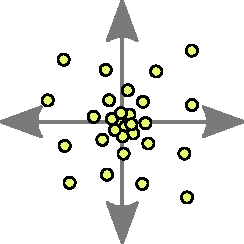
\includegraphics[scale=0.5]{Bilder/diffusion.pdf}
	&
      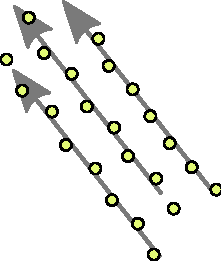
\includegraphics[scale=0.5,angle=-90,origin=c]{Bilder/advection.pdf}
	\\
    \end{tabular}

    \end{center}
    \hfill
    \begin{center}  
    
    {\tiny (\emph{Stochastic Problems in Physics and Astronomy}, Page 41, S. Chandrasekhar, 1943,
    \\[-0.15cm]
    Reviews of Modern Physics, American Physical Society)}
    
    \end{center}
    \end{frame}

    \begin{frame}
      \frametitle{Zeitschrittbeschränkung}
      Für Diffusion:
      $$\Delta t \leq \frac{\Delta x^2 \Delta y^2}{2D(\Delta x^2 + \Delta y^2)}$$
      
      \hfill
      
      {\tiny (\emph{pauli.uni-muenster.de/tp/fileadmin/lehre/NumMethoden/WS0910/ScriptPDE/Heat.pdf},
	  \\[-0.15cm]
      Page 12)}
      
      \hfill
      
      Für Advektion: "Vererbt" von Beschränkung für Strömungslöser
    \end{frame}

  \begin{frame}
    \frametitle{Gesamtgleichung}
    $$\frac{\partial s(\vec{x},s,t)}{\partial t} = \nabla \cdot (D \nabla s(t,\vec{x})) - \nabla \cdot (\vec{v}s) + R(\vec{x},s,t)$$
    
    Erweitert um allgemeinen Reaktionsterm R
  \end{frame}

  \section{Lotka-Volterra}
    \begin{frame}
    \frametitle{Lotka-Volterra-Modell}
    Reaktionsterm im Lotka-Volterra-Modell
    
    $$R(s,t) = \alpha_i s_i + s_i \sum_{j=1}^{n} \beta_{ij} s_j$$
    
    Zudem: $\beta_{ii} = -\frac{\alpha_i}{L_i}$ mit $L_i$ als Gleichgewichtspunkt
    
	\hfill    
    
    \begin{center}
    {\tiny (\emph{Principes de biologie mathématique}, V. Volterra, Acta Biotheoretica, 1937,
	\\[-0.15cm]    
    Volume 3, Issue 1, Pages 1–36)}
    \end{center}
    \end{frame}
    
    \begin{frame}
      \frametitle{Lotka-Volterra-Modell}
      \begin{itemize}
      \item Zwei Substanzen A: Beute, B: Jäger
      \end{itemize}
      \renewcommand{\arraystretch}{0.1}
      \setlength{\tabcolsep}{0.2em} % for the horizontal padding
      \begin{tabular}{ r c c c }
	  & Feed & Reaktion & Kill \\
	  &
      
\includegraphics[scale=0.12,angle=-90]{Bilder/lv_feed.pdf}
	  &
      
\includegraphics[scale=0.12,angle=-90]{Bilder/lv_mix.pdf}
      &
      
\includegraphics[scale=0.12,angle=-90]{Bilder/lv_kill.pdf}
	  \\
	  \(
		R_A(s_A,s_B)=
	  \)
	  &
	  \(
		\alpha_A s_A (L_A-s_A)
	  \)
	  &
	  \(
		- \gamma_A s_A s_B
	  \)
	  &
	  \\
	  \(
		R_B(s_A,s_B)=
	  \)
	  &
	  &
	  \(
		+ \gamma_B s_B s_A
	  \)
	  &
	  \(
		- \alpha_B s_B (L_B-s_B)
	  \)
	  \\
      \end{tabular}
      \renewcommand{\arraystretch}{1.0}
      \begin{itemize}
	  \item $\alpha_A$ Reproduktionsrate der Beute
	  \item $\gamma_A$ Fressrate der Räuber pro Beutelebewesen
	  \item $\gamma_B$ Reproduktionsrate der Räuber pro Beutelebewesen
	  \item $\alpha_B$ Sterberate der Räuber
      \end{itemize}
    \end{frame}
    
    \begin{frame}
    \frametitle{Verhalten \& Stabilität}
    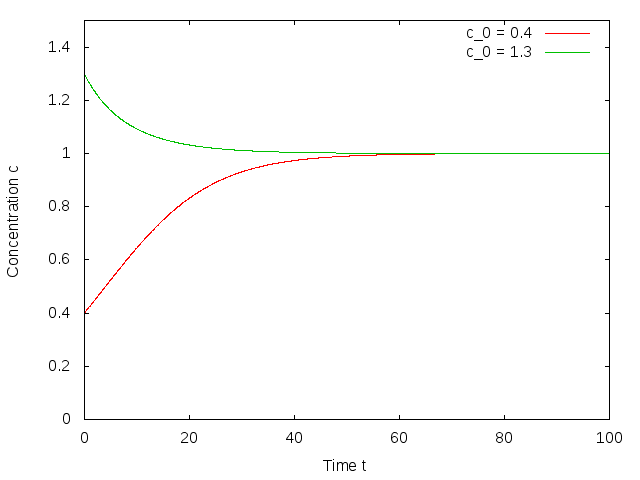
\includegraphics[scale=0.5]{Bilder/n1_anfangsbedingungen.png}
    \end{frame}
    
    \begin{frame}
    \frametitle{Verhalten \& Stabilität}
    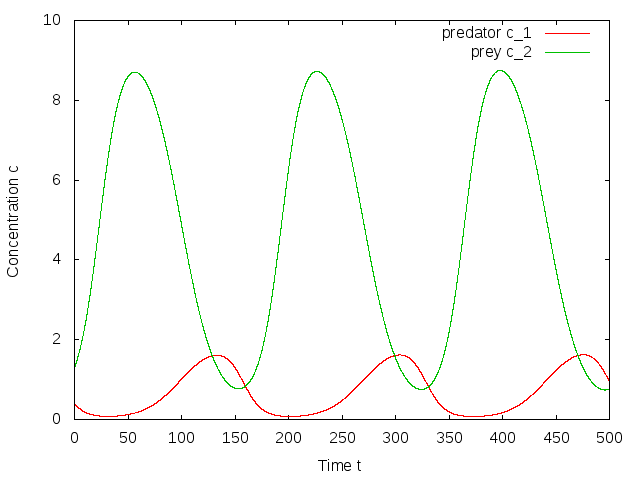
\includegraphics[scale=0.5]{Bilder/n2_unged_schwingungen.png}
    \end{frame}
    
    \begin{frame}
    \frametitle{Verhalten \& Stabilität}
    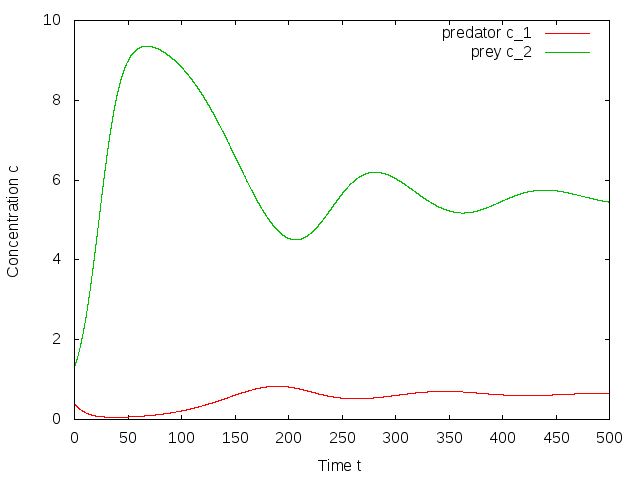
\includegraphics[scale=0.5]{Bilder/n2_ged_schwingungen.png}
    \end{frame}
    
    \begin{frame}
    \frametitle{Verhalten \& Stabilität}
    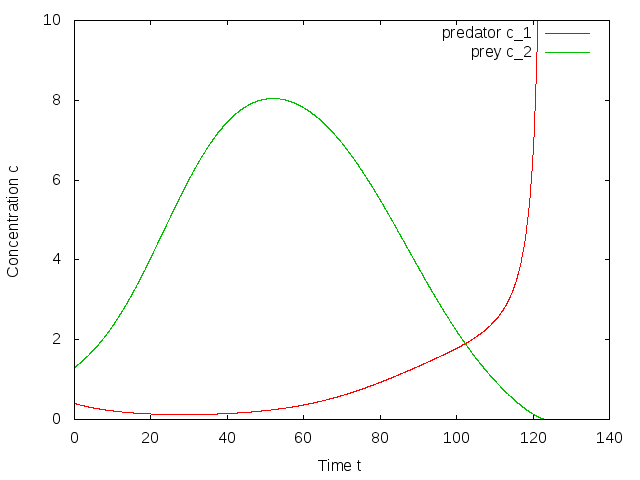
\includegraphics[scale=0.5]{Bilder/n2_explodiert.png}
    \end{frame}
    
    \begin{frame}
    \frametitle{Verhalten \& Stabilität}
    \begin{itemize}
      \item Instabilität durch Parameter und Löser überlagert
      \item Löser lässt sich durch symplektische Verfahren ersetzen
      \item Parameterwahl nicht trivial, aber auch nicht willkürlich
    \end{itemize}
    \end{frame}
    
    
    \begin{frame}
    \begin{center}
    \frametitle{Inspiration}
    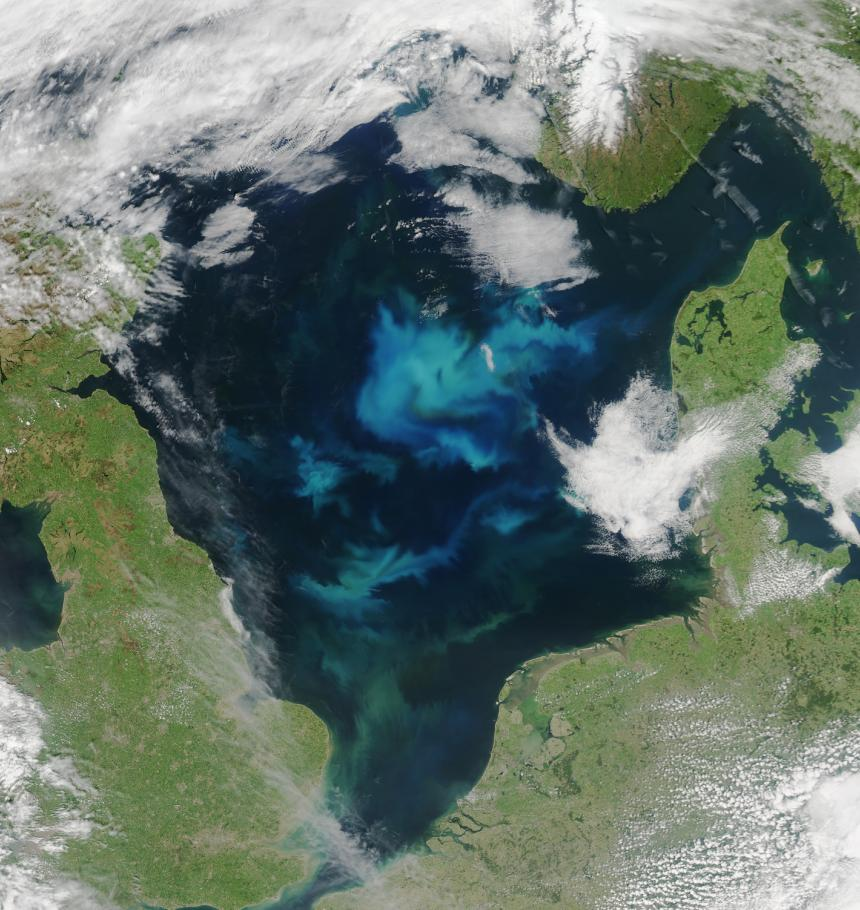
\includegraphics[scale=0.15]{Bilder/seaweed.jpg}
    
    {\tiny \textit{Quelle: http://www.spiegel.de/wissenschaft/natur/bild-1042982-869697.html}}
    \end{center}
    \end{frame}
    

    \section{Gray-Scott}
    
    \begin{frame}
      \frametitle{Idee des Gray-Scott Modells}
      \begin{itemize}
      \item Zwei Substanzen A: Futter, B: Räuber
      \renewcommand{\arraystretch}{0.1}
      \setlength{\tabcolsep}{0.2em} % for the horizontal padding
      \end{itemize}
      
      \begin{tabular}{ r c c c }
	  & Feed & Reaktion & Kill \\
	  &
      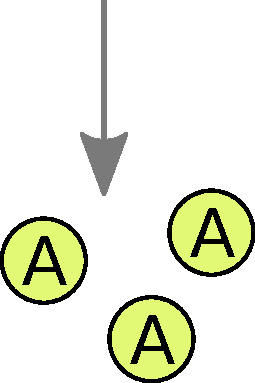
\includegraphics[scale=0.2]{Bilder/gs_feed.pdf}
	  &
      
\includegraphics[scale=0.2,angle=-90,origin=l]{Bilder/gs_reaction.pdf}
      &
      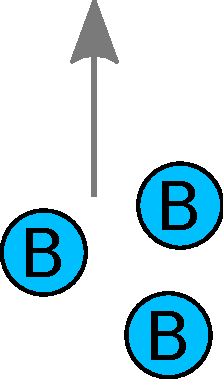
\includegraphics[scale=0.2]{Bilder/gs_kill.pdf}
	  \\
	  \(
		R_A(s_A,s_B)=
	  \)
	  &
	  \(
		f(1-s_A)
	  \)
	  &
	  \(
		- s_A s_B^2
	  \)
	  &
	  \\
	  \(
		R_B(s_A,s_B)=
	  \)
	  &
	  &
	  \(
		+ s_A s_B^2
	  \)
	  &
	  \(
		- (k + f) s_B
	  \)
	  \\
      \end{tabular}
      \renewcommand{\arraystretch}{1.0}

      \begin{itemize}
	  \item Kill-Rate $k$
	  \item Feed-Rate $f$
	  \item Diffusions-Konstanten $d_A, d_B$
      \end{itemize}
      
      {\tiny (\emph{Autocatalytic Reactions in the Isothermal Continuous Stirred Tank Reactor}, P. Gray and S. K. Scott, \\[-0.15cm]
    1984, Chemical Engineering Science)}
    
      \end{frame}

      \begin{frame}
      \frametitle{Gray-Scott Modell ohne Advektion}

      \begin{itemize}
	  \item Muster bekannt von
      \begin{itemize}
	  \item	Blättern
	  \item Tierfellen (Rehe, Giraffen, Schmetterlinge, ...)
	  \item Mitose
      \end{itemize}
      \end{itemize}
      \begin{tabular}{l}
	  
\includegraphics[width=\textwidth,keepaspectratio]{Bilder/gs_scenarios.png} \\
      \end{tabular}
      
      {\tiny (http://www.karlsims.com/rd.html)}

    \end{frame}

\end{document}
